\documentclass{article}
 
% if you need to pass options to natbib, use, e.g.:
% \PassOptionsToPackage{numbers, compress}{natbib}
% before loading nips_2016
%
% to avoid loading the natbib package, add option nonatbib:
% \usepackage[nonatbib]{nips_2016}

% \usepackage{nips_2016}

% to compile a camera-ready version, add the [final] option, e.g.:
\usepackage[final]{nips_2016}

\usepackage[utf8]{inputenc} % allow utf-8 input
\usepackage[T1]{fontenc}    % use 8-bit T1 fonts
\usepackage{hyperref}       % hyperlinks
\usepackage{url}            % simple URL typesetting
\usepackage{booktabs}       % professional-quality tables
\usepackage{amsfonts}       % blackboard math symbols
\usepackage{nicefrac}       % compact symbols for 1/2, etc.
\usepackage{microtype}      % microtypography
\usepackage{graphicx}
\usepackage{blindtext}

\graphicspath{{./report_images/}}
 
\title{10-701 Final Project}

% The \author macro works with any number of authors. There are two
% commands used to separate the names and addresses of multiple
% authors: \And and \AND.
%
% Using \And between authors leaves it to LaTeX to determine where to
% break the lines. Using \AND forces a line break at that point. So,
% if LaTeX puts 3 of 4 authors names on the first line, and the last
% on the second line, try using \AND instead of \And before the third
% author name.

\author{
  Michael Lee \\
  % Department of Computer Science\\
  % Carnegie Mellon University\\
  \texttt{ml5@andrew.cmu.edu} \\
}

\begin{document}
% \nipsfinalcopy is no longer used

\maketitle

\section{Left/Right Footprint Detection Using MNIST Architecture}

\subsection{Image Preprocessing}
The 10,000 training images of left and right footprints were always bounded by a rectangle of Gaussian noise and came in a variety of orientations and crops. The flexibility and expressivity of neural networks (which are essentially series of nonlinear functions) can both be its greatest strength but also its greatest weakness. While the objective in this problem was to learn distinguishing features of left and right footprints, a neural network may actually end up learning additional misleading features if trained on the raw data. For example, it might notice that left feet are more prone to be vertically oriented while right feet are more prone to be horizontally oriented, which is an artifact of our particular dataset. Therefore, all the training images and testing images were preprocessed in the following manner.

As all images were affected by Gaussian noise, first a mask of the footprint track (the area within the parallel boundaries between the Gaussian noise around the footprint and white background) was created. This was done by blurring the image with two median filters (of size 5x5 then 10x10) and finding all the pixels below the pixel brightness of 255 (which extracted the white background). A median filter was used in order to maintain as much of the sharp edge between the footprint track and the white background as possible. Using a simple averaging Gaussian filter would have allowed outliers to blur edges (if most of the pixels in the averaging filter consisted of the white background but a few were black, the result of the averaging filter be would be pulled to below 255, whereas a median filter would output 255 and properly classify as the background).

Then the edges of the mask were located using a Sobel filter, which combines the results from horizontal and vertical derivative operations which give rise to horizontal and vertical edges respectively. The longest edge was then found as the longest connected component in the edge image, which always corresponded to the edges of the track that paralleled the sides of the footprint. The image was then rotated using the angle between that edge and the y-axis of the image to be aligned vertically. (While this method for orienting the images wasn't perfect and it left the ambiguity of the foot pointing upward or downward, the neural network was able to determine the determine the difference between the left and right feet reasonably well).

The final steps of the preprocessing step involved cropping the image to only include the footprint track (without the background) and resizing the image into a common size to feed into a neural network. Though the average imension of the training images was found to be 470 x 230, the final preprocessed image size was reduced to 235 x 115 due to GPU memory constraints.

\begin{figure}[h]
  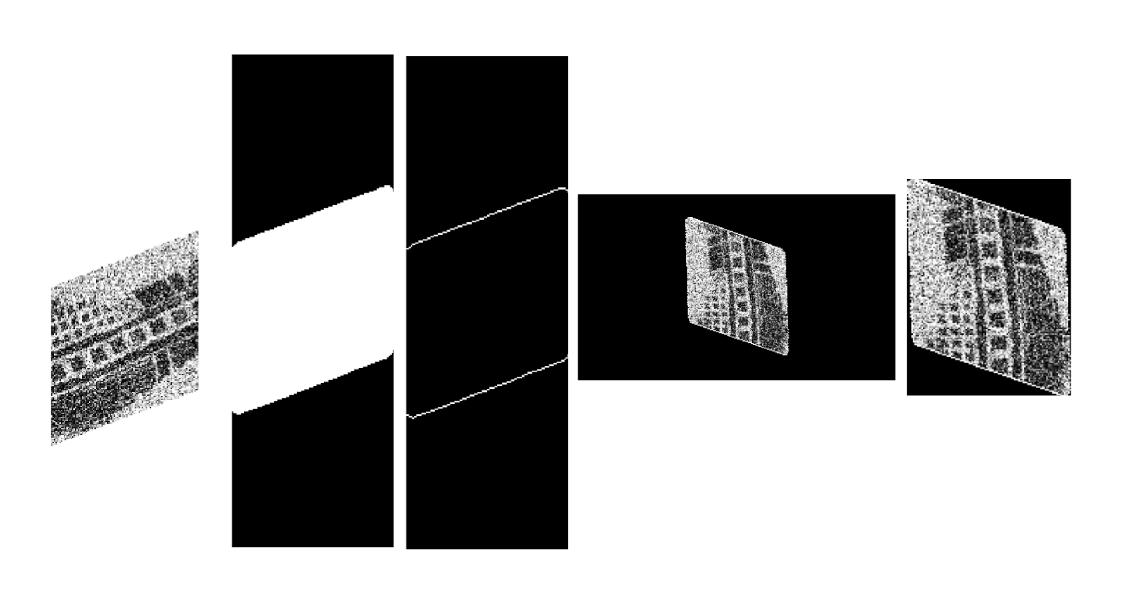
\includegraphics[width=\linewidth]{preprocessing_1.png}
  \caption{Image preprocessing steps: (From left to right) Original image, mask of footprint track, edges of footprint track, rotated image, cropped and rescaled final preprocessed image}
  \label{fig:preprocessing_1}
\end{figure}

\subsection{Learning algorithm}

\subsubsection{Library}
Keras with Tensorflow was selected due to its simple front-end interface and very powerful backend for designing and training neural networks. Though other learning algorithms could've been used, such as an SVM with an RBF kernel, I wanted to gain hands on experience with deep learning through this project.

\subsection{Network Architecture}
For the simple left/right classification, the original MNIST architecture was trained from scratch on the training data. The rationale for starting off with this architecture was that recent, more popular but complex networks for Imagenet like Alexnet were designed to do 1000 way classification would likely be too large and be likely to overfit. 

In the first few attempts of training, it was found that the training and validation accuracies were stuck at 69\% and 50\% respectively regardless of multiple changes, such as using the Alexnet architecture, adding additional layers, etc. It turned out that although the Adagrad weight update method is often preferred over Adadelta due to its greater robustness to intial learning rate, Adagrad performed very poorly on this dataset. Adagrad can perform better than Adadelta in a saddle point but Adadelta performs better at in an error manifold that resembles Beale's function (the large initial gradient makes Adagrad almost go unstable) and a long valley (Adadelta breaks the symmetry and descends much faster), which can be seen in Figure \ref{fig:optimizers}. Though the figures only represent canonical 2D error manifolds with no local minima, it still gives some insight as to how the various weight optimizers behave. The error manifold for this problem was probably ridden with many local minima that the more conservative Adagrad approach could not escape out of. And although Adam is a more general extension of Adadelta, it also failed to perform well with this dataset. 

\begin{figure}[h]
  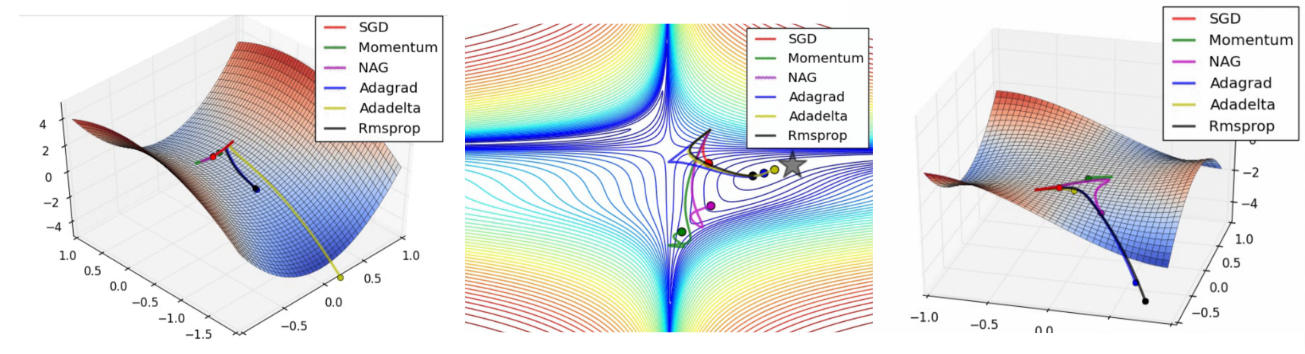
\includegraphics[width=\linewidth]{optimizers.png}
  \caption{Performance of popular weight optimizers in long valley, Beale's function, and saddle point scenarios (figures courtesy of Alec Radford, head of research at Indico Data Solutions)}
  \label{fig:optimizers}
\end{figure}

With a more suitable weight optimizer, the final architecture took the original MNIST architecture and added two back to back convolution layers after the max pooling layer, which is a common paradigm used in many Imagenet architectures like Alexnet and VGG. A final classification result of 94.2\% was achieved. 

% \begin{figure}[h]
%   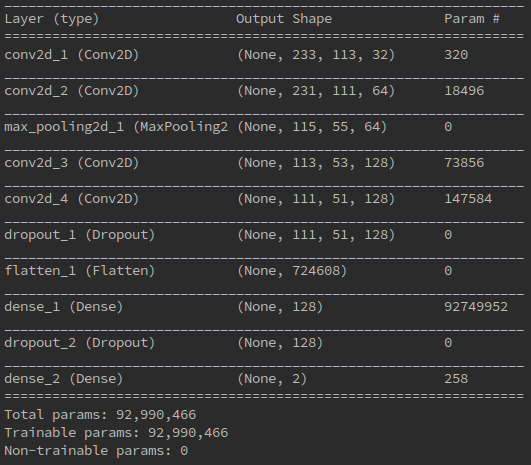
\includegraphics[width=\linewidth]{mnist_architecture.png}
%   \caption{Final network architecture for left/right footprint classification}
%   \label{fig:mnist}
% \end{figure}

\section{Footprint Matching}

\subsection{Image Preprocessing}

Image preprocessing of training and testing images were necessary due to the significant disparty between the two. While the original training images were always correctly oriented and the footprints were very clear with no noise, the testing images were peppered with Gaussian noise and oriented in arbitrarily. And while the testing images could either be of the left or right foot, the training images were always a right footprint.

Using the ImageDataGenerator class in Keras' library, each training image was resized into a standard size for training with a neural network and augmented into 20 additional images of a random orientation between 0 and 360 degrees with a random horizontal flip to become either left or right foot. The total training size increased from 1,000 images to 20,000 images.

The Gaussian noise from the test images were removed and the remaining foot print was made into a binary image to mimic the clean training images. 

\begin{figure}[h]
  \begin{center}
  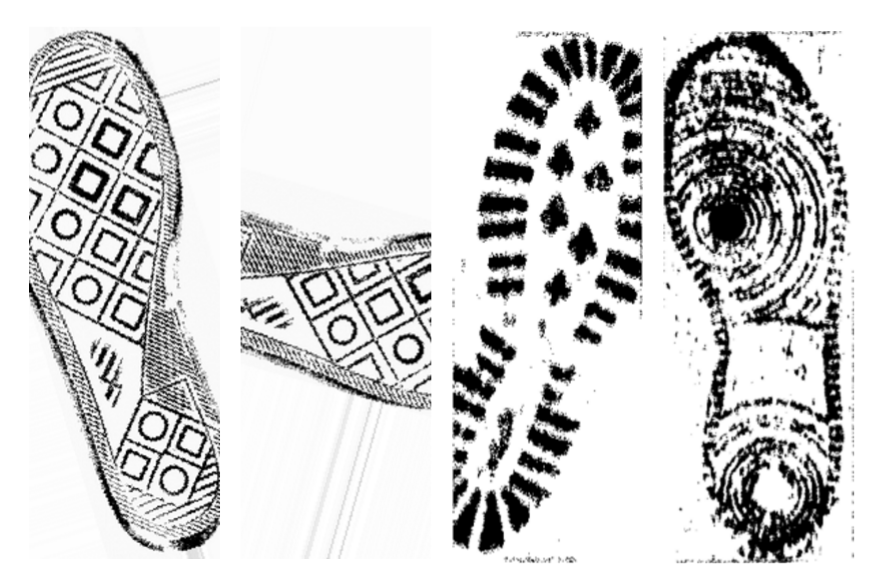
\includegraphics[width=0.5\linewidth]{2_preprocessing.png}
  \caption{(Left two images) sample augmentations of a training image that varies in orientation and left/right category (Right two images) instances of preprocessed test images}
    \end{center}
  \label{fig:preprocessing_2}
\end{figure}


\subsection{Architecture and Methods}

Inception v3 architecture was used as it posed a good compromise between accuracy and parameters on the Imagenet challenge (while having fewer parameters both VGG and Alexnet, it achieved higher performance). Three different training methods were tried.

\subsubsection{Training from Scratch}

The first method attempted trained the Inception architecture from scratch, under the rationale that the Imagenet weights would have learned to differentiate color in the RGB Imagenet images. The training data was split into a 70/30 train/validation split, which was carefully done so that the training and validation distributions were the same. This meant that 70\% of the augmented images for each of the 1000 classes were used for training and 30\% of the augmented images for validation, as opposed to a random 70/30 split over the entire 20,000 image dataset. However, after training for 12 epochs, the many of the 10,000 test predictions consisted of only a subset of the training images (for example, training image 812 was repeatedly predicted many times in a row).

This led to the hypothesis that the network was not expressive or deep enough.

\subsubsection{Additional Layers}

The next method involved inserting a couple dense layers at the top of the network to increase the network's ability to a more complex function. The training and validation results improved (achieving 95\% and 92\%) respectively, but it still performed poorly on test data, only achieving 0.1\% which corresponded to random guessing and suggested overfitting.

At this point, the test data was preprocessed to remove Gaussian noise and become binary, which brough up the test accuracy to 0.2\%. In order to try and prevent overfitting, transfer learning was tried next.

\subsubsection{Transfer Learning}

The original Inception v3 architecture was once more but it was now loaded with pretrained Imagenet weights. The first layer was changed however to accomodate grayscale images. The input images were resized to 224 x 224 to mimic the original Imagenet images.

This new network was trained for 6 epochs and achieved extremely good training and validation accuracies but failed to achieve a high test accuracy, indicating overfitting once again.

\subsection{Further Considerations}

In the end, the highest achieved test accuracy remained at 0.2\% with an Inception V3 base architecture trained from scratch with additional dense layers placed at the end.

Some additional techniques that would've been worthwhile to try include would include

\begin{itemize}
\item further preprocessing the images to get rid of some the solid black lines and rulers at the periphery of the image.
\item orienting the test images vertically so it's not left to chance that one of the 20 augmentations would be at the exact orientation as the one arbitrarily oriented test image
\end{itemize}

\section{Clustering}

PCA was used to cluster the images in the spirit of the work done in the 1987 paper Low-dimensional Procedure for the Characterization of Human Faces by Lawrence Sirovich and Michael Kirby. 

A preclustering step was first done to separate the images into full and partial images of feet by using the aspect ratio of the image's height to width. Clustering those with an aspect ratio greater than 2 as full feet and those with an aspect ratio of less than 2 as partial feet separated the dataset cleanly. The same clustering approach that will be outlined in the remaining pages was done for the full image and partial image datasets of 184 and 116 images respectively.

For each dataset, all images were vectorized and stacked on top of one another row-wise. Then each column of the data matrix was normalized to be zero mean and unit variance (corresponding pixels of all images being normalized to one another).

One common way to do PCA on a dataset is to find the eigenvectors and eigenvalues of the covariance matrix of the dataset. However, in this case, covariance matrix of each data matrix was severely rank deficient and limited by the number of samples in the full and partial image datasets (which is often much smaller than the number of pixels in each individual image). Therefore, instead of finding the eigenvectors and values of $XX^T$, a p x p matrix where p is the number pixels in each image, they were found for $X^TX$, an n x n matrix where n is the number of samples.

The acquired eigenvectors had the same dimensionality as the images and could themselves be visualized as images, as shown in Figure \ref{fig:eigenfeet}. Outlines of foot prints are clearly visible.

\begin{figure}[h]
  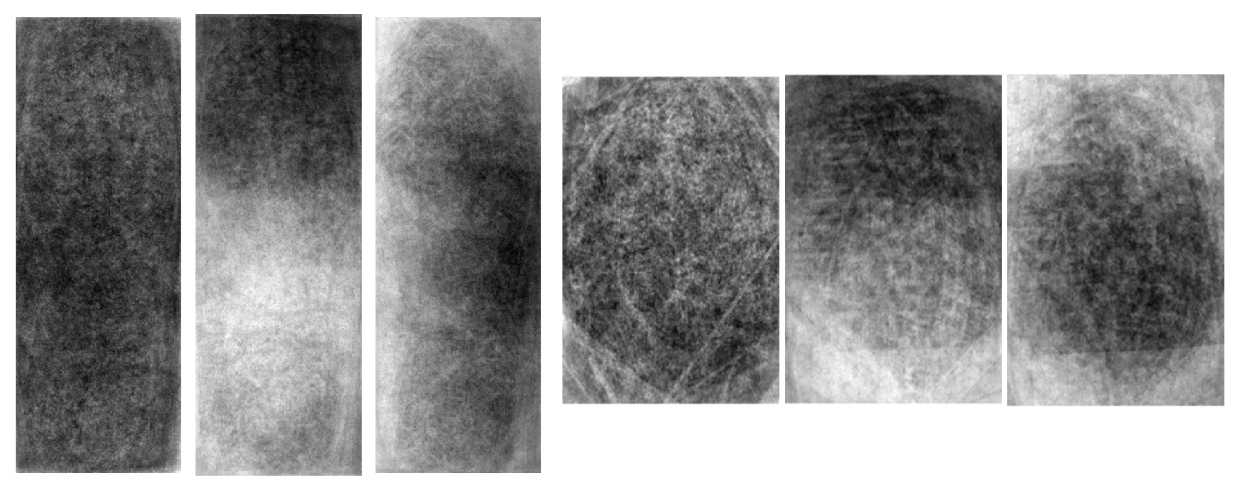
\includegraphics[width=\linewidth]{eigenfeet.png}
  \caption{Visualization of three principal bases for full (left three) and partial (right three) footprints }
  \label{fig:eigenfeet}
\end{figure}

Finally, new features were extracted for each image by summing the absolute differences between that image and all other eigenfaces and were used to do k-means clustering.

A cluster number of 10 and 7 respectively for the full and partial image datasets results in clusters like the ones demonstrated in Figures \ref{fig:full_cluster} and \ref{fig:partial_cluster}. Unfortunately the clusters seem to focus more on more macroscopic features such as overall color of the image and frequency of texture (high vs low) rather than specific pattern. 

\begin{figure}[h]
  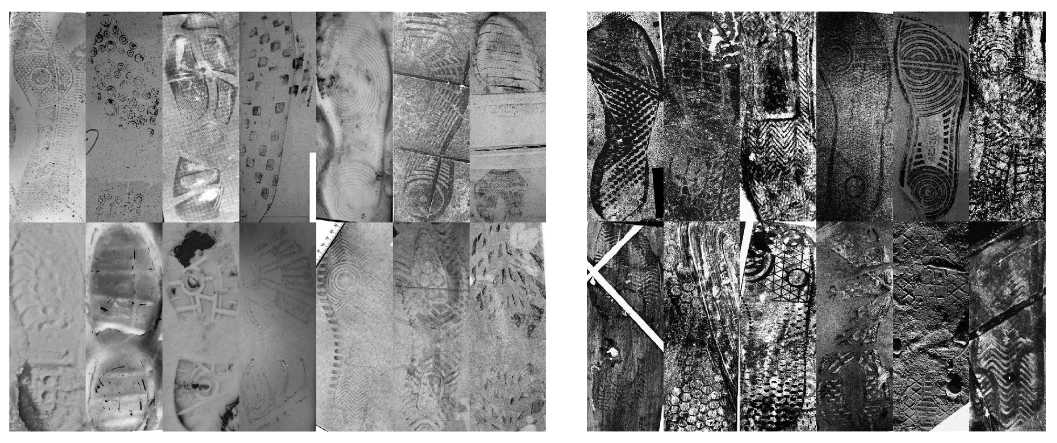
\includegraphics[width=\linewidth]{full_cluster.png}
  \caption{Two representative clusters produced for full foot images}
  \label{fig:full_cluster}
\end{figure}

\begin{figure}[h]
  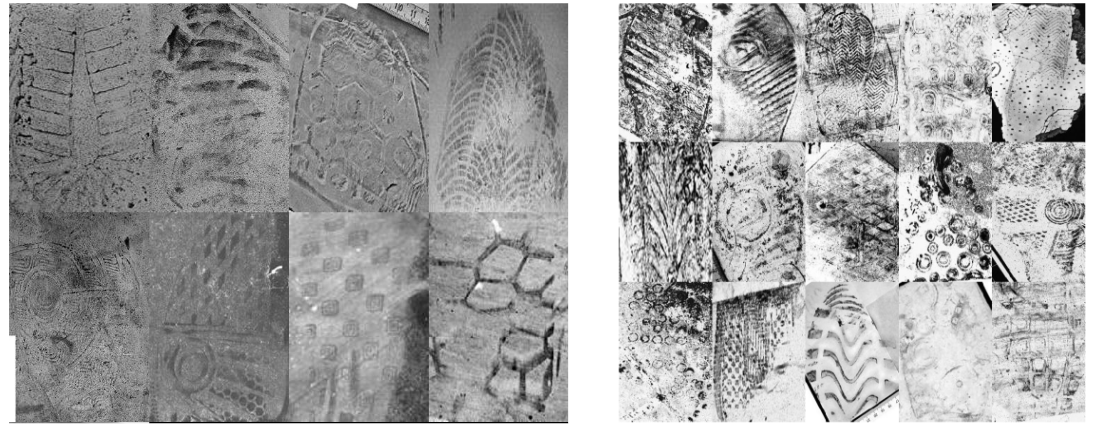
\includegraphics[width=\linewidth]{partial_cluster.png}
  \caption{Two representative clusters produced for partial foot images}
  \label{fig:partial_cluster}
\end{figure}



\end{document}
